\documentclass[a4paper,12pt]{article}
\usepackage{HomeWorkTemplate}

\usepackage[utf8]{inputenc}
\usepackage[]{babel}

\setlength{\parindent}{4em}
\setlength{\parskip}{0.5em}

\renewcommand{\baselinestretch}{1.5}


\usepackage{caption}
\usepackage{subcaption}
\usepackage{graphicx}
\usepackage{float}
\usepackage[utf8]{inputenc}
\usepackage{lmodern, textcomp}
\usepackage{circuitikz}
\usepackage[shortlabels]{enumitem}
\usepackage{hyperref}
\usepackage{tikz}
\usepackage{amsmath}
\usepackage{amssymb}
\usepackage{tcolorbox}
\usepackage{graphicx}
\usepackage{xepersian}
\settextfont{XB Niloofar}
\usetikzlibrary{arrows,automata}
\usetikzlibrary{circuits.logic.US}
\usepackage{changepage}
\newcounter{problemcounter}
\newcounter{subproblemcounter}
\setcounter{problemcounter}{1}
\setcounter{subproblemcounter}{1}
\newcommand{\problem}[1]
{
	\subsection*{
		پرسش
		\arabic{problemcounter} 
		\stepcounter{problemcounter}
		\setcounter{subproblemcounter}{1}
		#1
	}
}
\newcommand{\subproblem}{
	\textbf{\harfi{subproblemcounter})}\stepcounter{subproblemcounter}
}


\begin{document}
\handout
{اصول پردازش تصویر}
{دکتر مصطفی کمالی تبریزی}
{نیم‌سال اول 1399\lr{-}1400}
{اطلاعیه}
{سیدعلیرضا خادم}
{97100398}
 {تمرین سری اول - سوال سوم}
\section*{موارد لازم.}\label{n}
برای اینکه کد 
$ q_3.py $
به درستی اجرا شود، لازم است که تصویرِ ورودی با در مسیرِ 
\lr{EX1\_Q3/images/}
قرار بگیرد.بعد از اجرایِ کد از شما خواسته می‌شود که نام تصویر را همراه با فرمت آن وارد کنید، با وارد کردنِ نام تصویر ورودی و زدن کلید اینتر منتظر باشید تا کد اجرا شود و نتیجه در مسیرِ
\lr{EX1\_Q3/results/}
ذخیره شود.
\section*{روند کلی حل.}
ایده اصلی و روند کلی حل این سوال به این صورت است که، بعد از این که تصویر رقمی شده‌یِ ورودی را به سه قسمتِ افقیِ مساوی تقسیم کردم، برای هر یک از سه تصویر حاصل
\lr{edge detection}
انجام میدهیم تا مرزها در این سه تصویر مشخص شوند. با توجه با اینکه این عکس ها از یک منظره هستند مرزهای مشترک آنها  بسیار زیاد است و اگر بتوانیم این مرزهای مشترک را بر هم منطبق کنیم توانسته‌ایم این سه عکس رو به درستی رو هم قرار دهیم و نتیجه مطلوب را به دست آوریم. برای این که این کار را انجام دهیم یکی از این سه عکس را به عنوان مرجع در نظر میگیریم و هر سه عکس را روی این عکس با روش 
\lr{sum of squared differences}
سرچ می‌زنیم. و با توجه به نتایج میزان جابه‌جایی ها رو محاسبه می‌کنیم.\\
ما در این سوال کانال آبی را به عنوان مرجع در نظر می‌گیریم و سه کانال را روی این کانال سرچ میزنیم. با فرض ثابت بودن کانال آبی جابه‌جایی کانال‌های سبز و قرمز به صورت زیر خواهد بود.
\begin{align*}
	&\Delta X_G = 9 , \Delta Y_G = 88 \\
	&\Delta X_R = 12 , \Delta Y_R = 181
\end{align*}


\section*{توضیح کد.}
\subsection*{$\circ$ utilities.py}
\subsubsection*{split\_image\_horizontally}
این تابع یک عکس و  عدد
\lr{t}
 را به عنوان ورودی می‌گیرد و عکس را افقی، به 
 \lr{t}
  قسمت مساوی تقسیم می‌کند و  قسمت‌ها را در یک آرایه می‌ریزد و به عنوان خروجی این آرایه را برمی‌گرداند.
  \subsubsection*{edge\_detection\_filter}
  این تابع یک عکس به عنوان ورودی می‌گیرد و فیلتر
  \lr{edge detection}
  را روی این عکس اعمال می‌کند و نتیجه را با یک 
  \lr{threshold}
  باینری کرده و برمی‌گرداند.
  \subsubsection*{ssd}
  این تابع یک عکس ، یک تمپلیت و عدد 
  \lr{k}
  را به عنوان ورودی می‌گیرد و با توجه به روابط زیر 
  \lr{SSD}
  را محاسبه می‌کند.\\
  \begin{figure}[H]
  	\centering
  	\begin{subfigure}{0.9\textwidth}
  		\centering
  		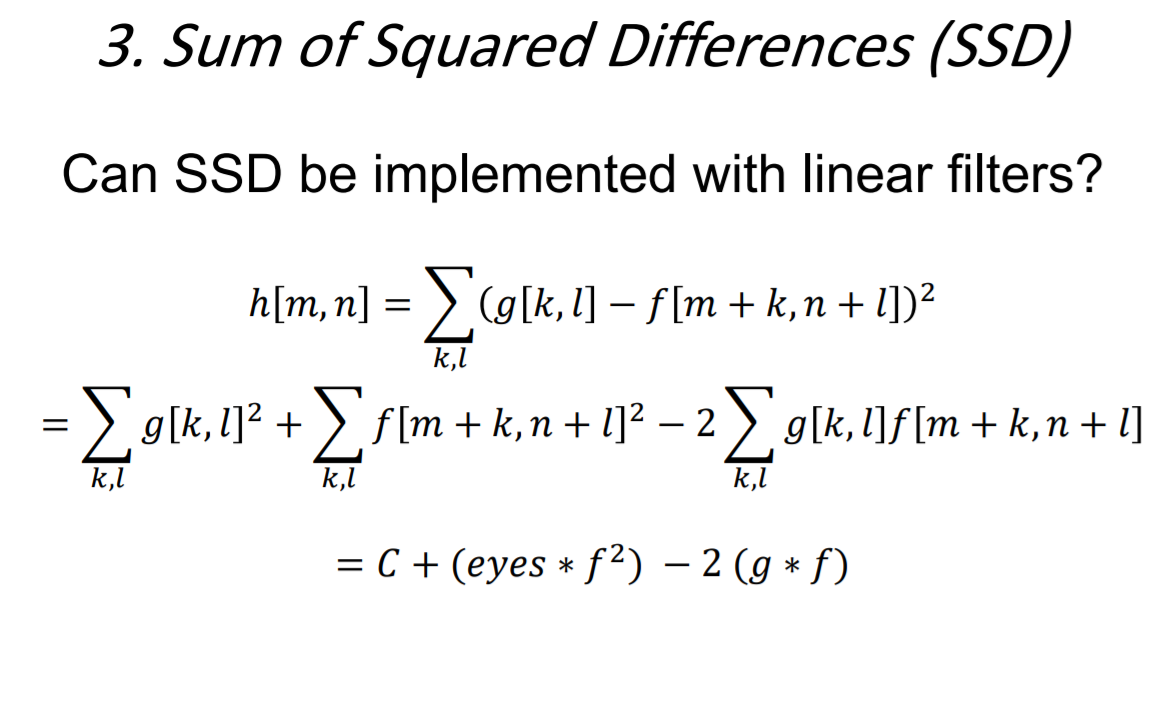
\includegraphics[width=\textwidth]{1.png}
  	\end{subfigure}
  \end{figure}
با این تفاوت که ثابت 
\lr{C}
را محاسبه نمی‌کنیم و به تبع آن همه مقادیر را منهایِ مینیمم میکنیم تا مقدار منفی نداشته باشیم و به اضافه 1.1 می‌کنیم تا حداقل مقدار در  
\lr{result}
1.1 
باشد و بعد که میخواهیم لگاریتم بگیریم اعداد منفی نداشته باشیم و به مشکل نخوریم. بعد هم چون اعداد
\lr{result}
 خیلی بزرگ می‌شوند 
 \lr{k}
 بار لگاریتم می‌گیریم تا بتوانیم با این اعداد راحت تر کار کنیم. در نهایت هم مینیمم مقدار 
 \lr{result}
 را به عنوان نقطه‌ای که متچینگ انجام شده برمی‌گردانیم.
 \subsubsection*{get\_image\_name}
 این تابع با چاپ کردنِ عبارتِ
 \lr{"please enter name of image with its format"}
 از کاربر میخواهد تا نام عکسی که به عنوان ورودی قرار است به برنامه داده شود را همراه با فرمت تایپ کند. و بعد نامی که کاربر وارد کرده است را برمی‌گرداند.
\subsection*{$\circ$ q3.py}
در این فایل ابتدا نام تصویر از کاربر گرفته می‌شود و تصویر لود می‌شود. بعد تصویر به سه قسمت مساوی تقسیم می‌شود و روی هر کدام از این قسمت‌ها
\lr{edge detection}
انجام می‌دهیم.
\lr{edf\_channel}
و
\lr{eds\_channel}
و 
\lr{edt\_channel}
را با روش 
\lr{sum of squared differeces}
رویِ
 \lr{edf\_channel}
 سرچ می‌زنیم. بعد با نتایجی که به دست می‌آوریم و با ثابت فرض کردنِ کانالِ آبی میزان جابه‌جایی کانال‌هایِ سبز و قرمز را مجاسبه می‌کنیم و با استفاده از 
 \lr{Geometric Transformations}
 آن ها را جابه‌جا می‌کنیم. نیتجه از مرج کردنِ سه کانال حاصل می‌شود. در نهایت هم با توجه به اینکه حاشیه‌ها 
 \lr{pixel}
 هایی هستند که مقدار 
 \lr{intensity}
 یِ چنلِ آبی یا سبز یا قرمز در آنها نزدیک به 255 است، حاشیه‌ها را حذف میکنیم و با تغییر عکس به 
 \lr{unit8}
 آن را با فرمتِ 
 \lr{.jpg}
 در مسیرِ
 \lr{EX1\_Q1/results/}
 ذخیره می‌کنیم.
 
  
\end{document}
